\documentclass[12pt]{article}
\usepackage{graphicx} % Required for inserting images
\usepackage[numbers,square]{natbib}
\usepackage{rotating}
\usepackage{tabularx}
\usepackage{booktabs}
\usepackage{multirow}
\usepackage{subcaption}
\usepackage{placeins}
\usepackage{amsmath}
\usepackage{stfloats}
\usepackage{caption}
\usepackage{pdflscape}
\usepackage{graphicx}
\usepackage{adjustbox}
\usepackage{placeins}
\usepackage[
    a4paper,
    top=2cm,
    bottom=2.5cm,
    left=2cm,
    right=2cm
]{geometry}

\newgeometry{margin=2cm}
\begin{titlepage}
    \begin{center}
    \vspace*{\fill}

    {\large\bfseries Surrogate Model for Forecasting Hydrogen Storage Deliverability Using Deep-Learning.\par}
    \vspace{0.3cm}
    {\Large\itshape Project Plan\par}
    \vspace{0.5cm}
    {\normalsize\bfseries Thomas Peach\par}
    {\small\itshape MSc Geo-Energy with Machine Learning and Data Science\par}
    {\small\itshape https://github.com/ese-ada-lovelace-2025/irp-tlp25\par}

    \vspace*{\fill}

    Supervised by:\\[0.3cm]
    {\normalsize\bfseries Prof. Samuel Krevor\par}
    {\small\itshape Primary Supervisor\par}
    \vspace{0.5cm}
    {\normalsize\bfseries Dr. Adriana Paluszny\par}
    {\small\itshape Secondary Supervisor\par}

    \vspace*{\fill}

    
\includegraphics[width=0.4\textwidth]{IC_New_Logo.pdf}\\
    \vspace{0.5cm}
    {\normalsize Department of Earth Sciences and Engineering\par}
    {\normalsize Imperial College London\par}
    {\normalsize \today\par}

    {\normalsize Word Count = 1496 Words}

    \vspace*{\fill}
    \end{center}
\end{titlepage}

\newpage
\begin{document}

\section{AI Acknowledgements}
I used Anthropic's Claude Sonnet 4.6 for creation of tables, the title page in Overleaf and debugging the baseline model, all content within the tables was written by myself. The submitted work is my own and reflects my own understanding. The writing is all written by myself in my own words, and is inline with the Academic Integrity Declaration.

\section{Abstract}
This project aims to investigate a key issue within Underground Hydrogen Storage (UHS), the effect of different cycle lengths on hydrogen deliverability. Renewable energy supply varies significantly both on a seasonal and day-night time scale. This can result in excess energy being produced which is wasted, UHS solves this issue. Excess energy is used to produce hydrogen through electrolysis of water which is then stored underground until required. There are currently no operational UHS sites, as a result research has focussed on developing surrogate models using deep-learning methods. These are developed through the generation of large datasets in full-physics simulators which cover a range of uncertain variables. These datasets are then used to train deep-learning models. Existing research all focuses on using constant injection and withdrawal cycle lengths. This project will develop a forecasting model to predict hydrogen deliverability based off a dataset with varied injection and withdrawal cycle lengths.       

\section{Problem Description}
As we transition away from fossil fuels, renewable energy sources are growing dramatically. With this in mind and the fact that energy demand globally varies significantly, a stable base load supply of clean energy is crucial. One solution for this is underground hydrogen storage (UHS). This can be done in salt caverns, depleted gas fields and aquifers. Excess energy, ideally from renewables, is used to produce hydrogen via electrolysis of water. This is then pumped underground until required. The focus of this project will be on forecasting deliverability from depleted gas fields. In order for hydrogen storage sites to be operable and gain contracts, they need to be able to forecast the amount of energy they can supply.

\subsection{Significance}
In order for operators of future hydrogen storage sites to secure contracts to supply energy they need to be able to forecast the hydrogen that is deliverable from storage. This research proposes to generate synthetic data from reservoir modelling software. The research will use a pre-existing benchmark model created by \citet{hogeweg2022benchmark}. The dataset will be formed by altering the injection and withdrawal cycle lengths in the model, using natural gas cycle lengths as an analogue. Deep learning models such as Long Short-Term Memory networks (LSTMs) will then be used to forecast the future deliverability of a hydrogen storage site. This will allow for context from previous cycles to be included in forecasting deliverability. This is crucial for hydrogen storage to be integrated into the grid at scale.  

\subsection{Review of Existing Work}

The need for UHS is due to the seasonal and day-night variations in energy production from renewable energy sources, such as wind and solar. The variations lead to peak supply and demand being imbalanced which can result in energy being wasted, negative prices and grids being unstable \cite{pellow2015hydrogen}. UHS would be used to mitigate this imbalance. Hydrogen is produced from excess energy generated by renewables through electrolysis of water and then stored underground. This creating a stable base load supply of energy. As a result, the effects of changing the injection and production cycle lengths need to be explored due to the seasonal and day-night variations in energy production from renewables. This is the key focus of this research, investing the effects of varied injection and production cycle lengths.

Currently there are only two applications of UHS in depleted gas fields, the Diadema project in Argentina and the 'Underground Sun Storage 2030' project in Austria. Both of these cases are yet to be fully operational. As a result, there is no real world data which can be used to develop deep learning models. Current research investigating the application of deep learning models has been done by generating synthetic datasets. Typically the datasets are generated by defining a range of uncertain parameters based off existing literature and then sampling to cover the entire range. These sampled parameter values are then inputted into full-physics reservoir simulators  e.g.\ \citep{mao2024efficient, MAOcushion, mao2025deep, fu2025deep, du2025combining, chellal2025quantitative}. The sampled values are then used as the input parameters for the deep learning model with the target being the output from the full-physics reservoir simulations. The focus of existing research is summarised with the key output metrics and model architectures used in table \ref{tab:related_works}. 

\begin{table}[h]
\centering
\caption{Summary of Existing Research on Deep-Learning Applications to UHS}
\begin{tabularx}{\textwidth}{@{}p{1.5cm} X X X X @{}}
\toprule
\textbf{Study} & \textbf{Research Focus} & \textbf{Key Output Metrics} & \textbf{Deep-Learning Architecture} & \textbf{Storage Cycle Lengths} \\
\midrule
\citet{mao2024efficient} & Development of reduced-order models & Hydrogen Production Efficiency, Mole Fraction of H$_{2}$ in produced gas, Produced Gas to Water volume ratio & 3 Feed-Forward Networks outputting each metric individually & 10 cycles; 6-month injection period, 6 month withdrawal period per cycle\\[6pt]
\citet{MAOcushion}& Effects of different cushion gases & $H_2$ withdrawal efficiency, Produced $H_2$ purity, Produced Gas-Water Ratio, Well Injectivity & One Feed-Forward Network & 10 cycles; 6-month injection period, 6 month withdrawal period per cycle\\[6pt]
\citet{mao2025deep}& Comparison of deep learning architectures on 2D Data & Spatial Map of $H_2$ saturation or reservoir pressure & U-Net, Fourier Neural Operator and Segmentation Transformer & 10 cycles; 6-month injection period, 6 month withdrawal period per cycle\\[6pt]
\citet{fu2025deep}& 2D UHS Surrogate Models & Spatial map of reservoir pressure or $H_2$ saturation & Swin-Unet (Transformer based architecture with a U-Net Structure) & 10 cycles; 6-month injection period, 6 month withdrawal period per cycle\\[6pt]
\citet{du2025combining}& Optimizing key UHS parameters & $H_2$ production rate, dissolution rate, storage mass & XGBoost, Feed-Forward Network, CNN and LSTM & 6 cycles, each cycle has 5 month injection period, 1 month shut-in period and 6 month production period \\
\citet{chellal2025quantitative}& Fault Reactivation Surrogate Models & Maximum shear to normal stress ratio acting on the fault & 3 Feed-Forward Networks for 3 stress regimes: normal, strike slip and reverse faulting  & 10 cycles; 6-month injection period, 6 month withdrawal period per cycle\\
\bottomrule
\end{tabularx}
\label{tab:related_works}
\end{table}


The existing research papers so far all use consistent injection and production cycle lengths across their entire datasets. The majority of the papers use a 6-month injection period followed by a 6-month withdrawal period based off work by \citet{malki2024operate}. The use of a consistent cycle length is a key limitation for the existing research, acknowledged by \citet{malki2024operate}. The limitation derives from the need for UHS.

\subsection{Objectives}
This project will investigate the effects of varied injection and production cycle lengths on hydrogen storage deliverability. The key objectives are defined below:
\begin{itemize}
    \item Statistically characterise natural gas cycle lengths and use this as a proxy for cycle lengths in UHS to create a dataset. 
    \item Compare and develop deep-learning based models that forecasts hydrogen storage deliverability. Hydrogen production rate and efficiency (ratio of injection hydrogen to produced hydrogen ratio) will be the forecasted metrics. 
    \item Compare deep-learning models trained on constant cycle lengths against variable cycle lengths.
\end{itemize}

\FloatBarrier

\section{Methodology}
\subsection{Dataset Generation and Preprocessing}
The dataset will be generated using a similar approach to existing research as defined above. \citet{hogeweg2022benchmark} produced an open-source baseline reservoir model which represents an example UHS site which will be used to create the dataset in SLB's Eclipse reservoir simulator. The baseline model consists of 44652 grid cells (61 x 61 x 12) with each x and y cell representing 50m, the height is variable. Before the baseline model is altered to generate the dataset, the results from \citet{hogeweg2022benchmark} will be reproduced. The primary parameters that will be altered are the injection and production cycle lengths, all other parameters will be kept constant. 

The dataset encompassing a range of cycle lengths is crucial for the project's success. The parameter space for cycle length will be developed by statistically characterizing natural gas storage cycle lengths. This is done due to UHS likely being operated in a similar way to underground natural gas storage \cite{tarkowski2019underground}. A minimum and maximum range for injection period length, idle period length and production period length will be defined. From these ranges, samples will be generated using Latin Hypercube Sampling to ensure that the dataset is evenly distributed. This sampling method is used to ensure the parameter space is covered evenly which is needed to ensure the deep-learning model generalises to the entire parameter space. 

After the dataset scripts have been generated they will be ran on Imperial Colleges's HPC. The models will be ran on SLB's Eclipse simulator which the Imperial College Earth Science and Engineering department have a license for. The Eclipse simulator was chosen due to the baseline model source code being made available and has a faster run time per simulation than the DuMu$^x$ simulator, the alternative software used by \citet{hogeweg2022benchmark}. This is crucial for this research project as being able to generate a large dataset is key to training deep-learning models with strong performance. This does limit the options in accessing the effects of microbial activity on hydrogen storage; however, this is beyond the focus of this research project. The outputs from the Eclipse simulator will then be copied to the local drive and preprocessed. The preprocessing stage has two key steps; feature engineering and normalization. Feature engineering will be used to generate the efficiency parameter, one of the defined key metrics. Normalization of all model input and output data will be done to support the model training and forecasting. A Python script will be developed to ensure that the processing and addition of simulation results is both consistent and efficient.  

\subsection{Deep-Learning Model Development}
The deep-learning model development stage will establish a baseline model which can be used to compare differing model architectures. The baseline model will mirror model architecture in the existing literature, specifically Feed-Forward Networks (FFNs) similar to those used by \citet{mao2024efficient, MAOcushion, chellal2025quantitative}. However, FFNs are unlikely to be the highest performing model due to the nature of the research problem and the input data that will be used. Deep-learning architectures that deal with sequential data are likely to give much stronger results. As a result, different architectures based on the literature, such as LSTMs and Swin-Unet, will be used and compared. The testing and validation of the models will involve performance metrics such as $R^2$ and MAE. In addition, the results will be tested in the context of the study to investigate if predictions are physically realistic.

\section{Future Plan}
There are five stages to the future plan which are broken down in figure \ref{fig:GANTT}. The key stages are the dataset generation, model development and report writing with approximately a month for each of these stages. The validation of the \citet{hogeweg2022benchmark} has been completed and can be seen in figure \ref{fig:val_graph}.

\begin{figure}
    \centering
    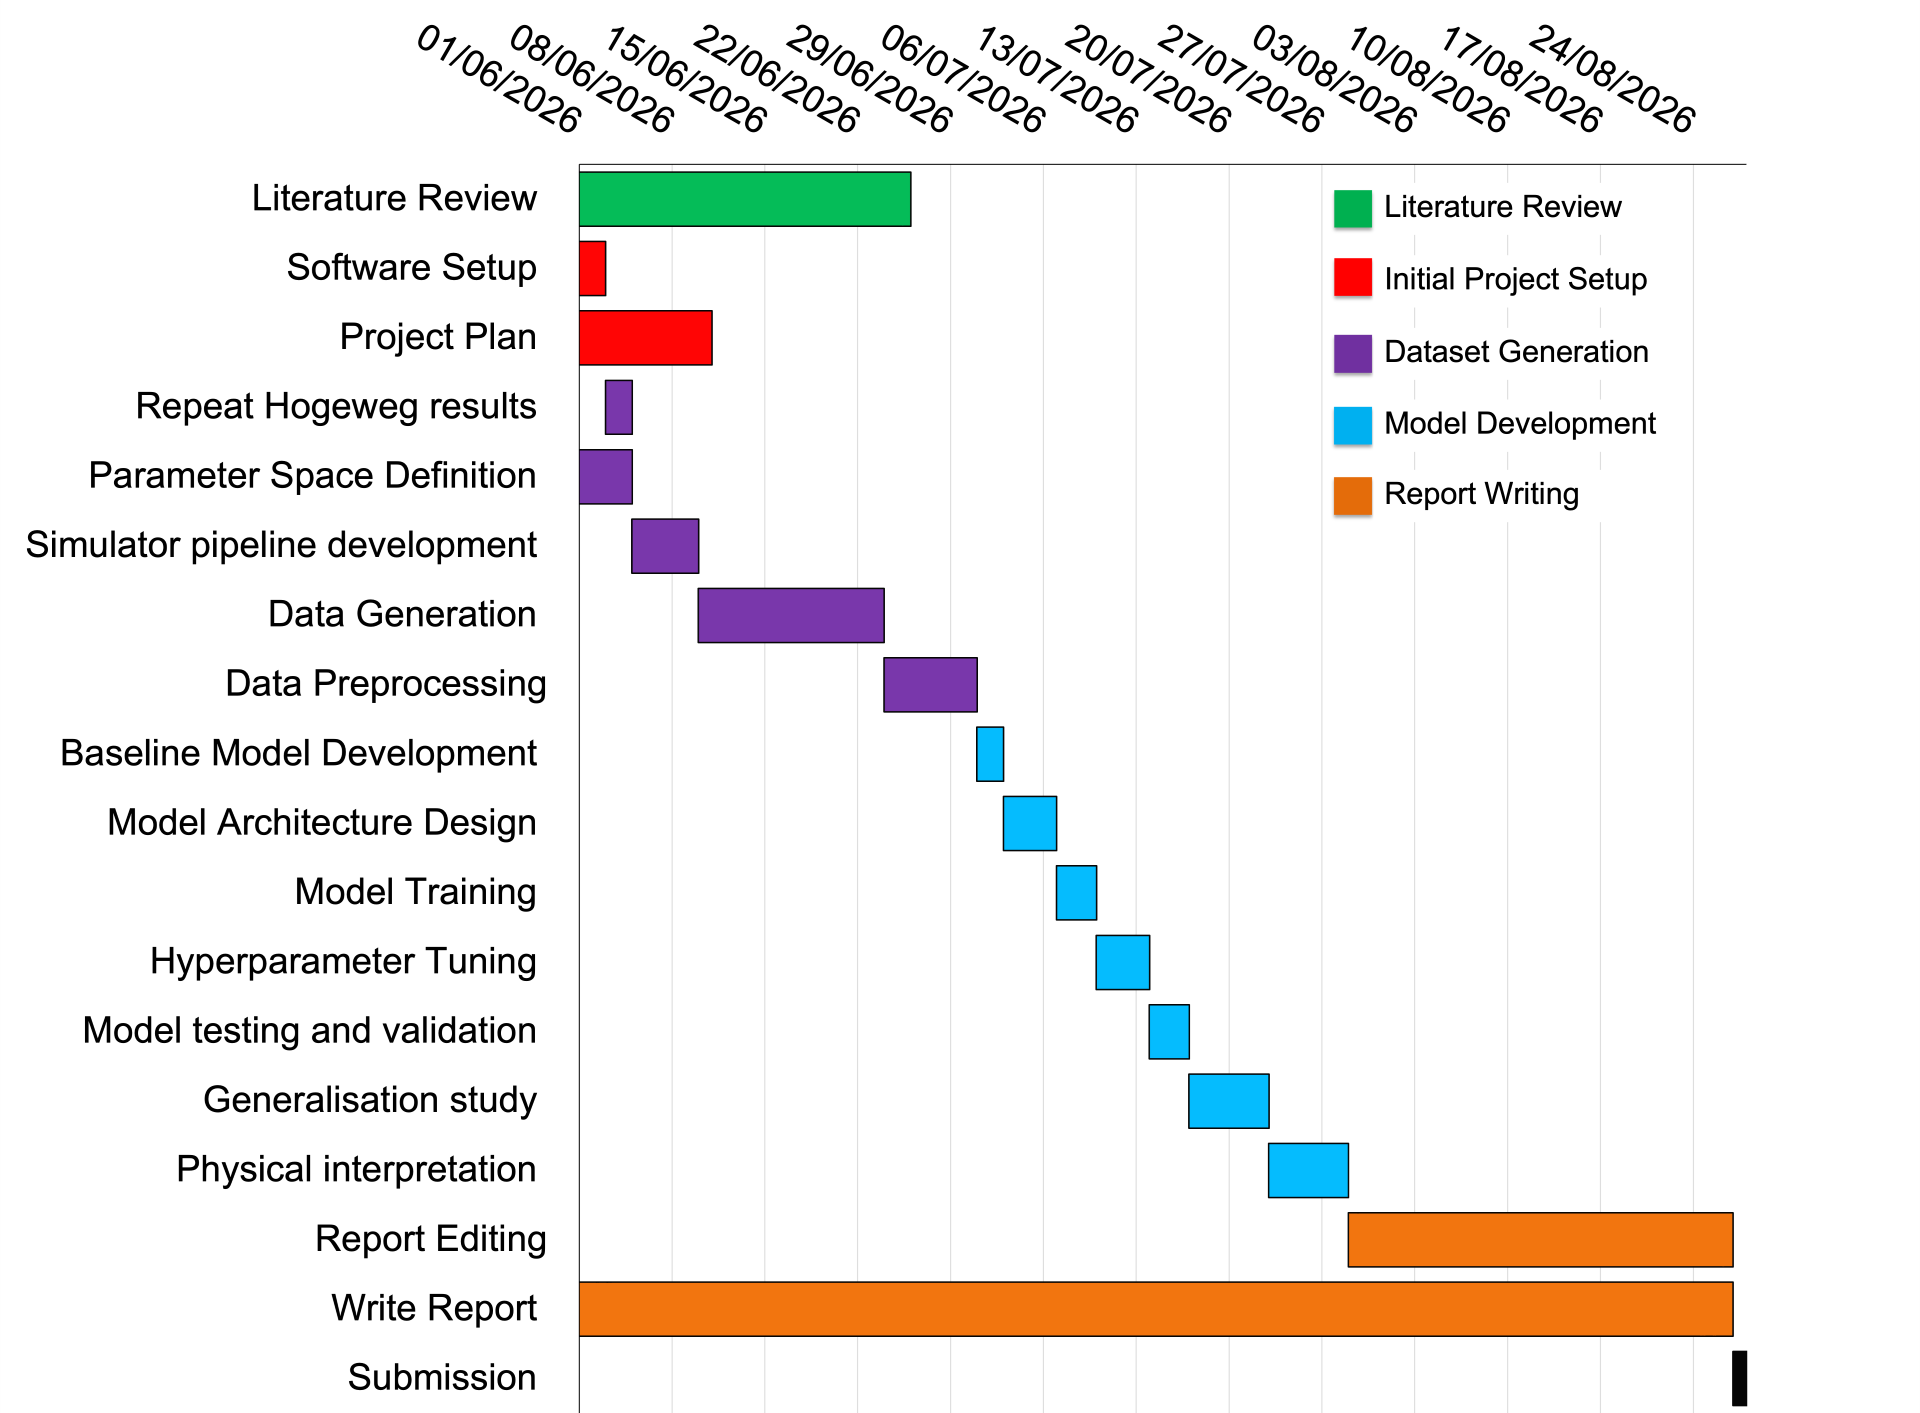
\includegraphics[width=1.1
    \linewidth]{IRP_GANTT.png}
    \caption{Gantt Chart for IRP timeline.}
    \label{fig:GANTT}
\end{figure}

The risks associated with the project are during the dataset generation phase and summarised in table \ref{tab:risk_mitigation}. The first risk is due to the baseline model being ran on the 2019 version of eclipse; however, Imperial's HPC only has the 2024 version available. This results in the simulation output to initially differ from the \citet{hogeweg2022benchmark} paper results. This is resolved by changing the data script to be compatible with the calculations used in the 2024 Eclipse version.

\begin{table}[h!]
\centering
\caption{Risk and Mitigation Strategies}
\label{tab:risk_mitigation}
\begin{tabular}{p{0.3\textwidth} p{0.6\textwidth}}
\toprule
\textbf{Risk} & \textbf{Mitigation} \\
\midrule
Baseline model is not compatible with SLB's Eclipse version on HPC & Edit Baseline model file to be compatible with new version or download older Eclipse software versions  \\
\addlinespace
Large dataset is not possible due to simulator runtimes & Use alternative machine learning approaches which do not require as large dataset\\
\addlinespace
Full dataset is not available till after estimated deadline & Build pipeline that allows results to be quickly preprocessed and added to dataset or use alternative machine learning approaches \\
\bottomrule
\end{tabular}
\end{table}

\begin{figure}
    \centering
    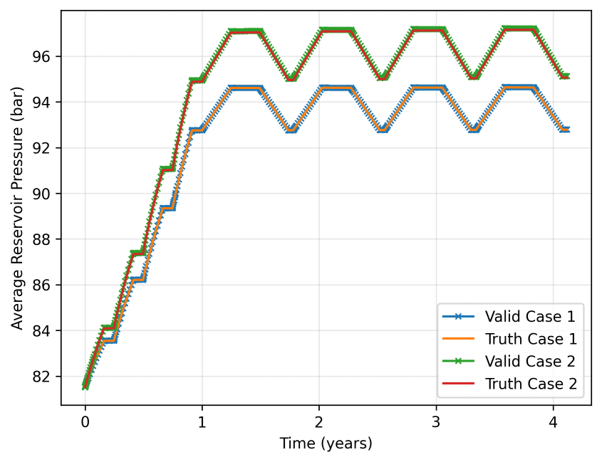
\includegraphics[width=0.7
    \linewidth]{Val_graph.png}
    \caption{Validation of \citet{hogeweg2022benchmark} results. Truth indicates the original results, valid represents the reproduced results.}
    \label{fig:val_graph}
\end{figure}

\FloatBarrier



\bibliographystyle{unsrtnat}
\bibliography{references}


\end{document}
